\RequirePackage{fix-cm}

\documentclass[smallextended,natbib]{svjour3}

\smartqed

\usepackage{graphicx}
\usepackage{amsmath}
\usepackage{booktabs}
\usepackage{placeins}
\usepackage{url}

\journalname{Empirical Software Engineering}

\begin{document}

\title{Monolith vs. Microservices Under Stress: A Controlled Benchmark of Fault Propagation, Latency, and Database Contention
	\thanks{The authors would like to thank Dr. Ahmed Warad and Associate Professor Dr. Kareem Kamal for their guidance and support.}
}

\titlerunning{Monolith vs. Microservices Under Stress}

\author{Bahaa El Deen Mohamed \and Ahmad Louay \and Youssef Khaled}

\authorrunning{Bahaa El Deen et al.}

\institute{Bahaa El Deen Mohamed \and Ahmad Louay \and Youssef Khaled \at
	Faculty of Computers and Information, Sadat Academy for Management Sciences, Cairo, Egypt \\
	\email{bahaa.abdelmoniem.fci2023033@sadatacademy.edu.eg}
}

\date{Received: date / Accepted: date}

\maketitle

\noindent\textbf{Clinical trial number:} not applicable.

\begin{abstract}
	While Microservices are widely adopted for large-organizational scalability and service autonomy, decomposition can introduce some drawbacks such as latency, failure-propagation, and data-tier coordination costs. This paper presents a controlled benchmark of monolithic and microservices implementations of the same e-commerce workload under equivalent business logic, identical datasets, and equivalent compute power. The evaluation covers four scenarios: baseline load, deterministic endpoint failure, fixed latency injection, and database connection pool stress. Apache JMeter was the tool used to perform stress tests and to gather and analyze data both during execution and across different scenarios, using metrics such as throughput, latency percentiles, error rates, confidence intervals, architectural changes, and performance degradation relative to the baseline.
	The results show a noticeable baseline efficiency advantage for the monolithic architecture in this environment, while the microservices architecture shows greater cascading effects under stress conditions during complex order-processing operations. Latency injection produces the largest degradation in both architectures; aggregate P95 inflation is larger for the monolith, while microservices exhibits higher overall error and stronger order-path failure amplification. Pool-size sweeps reveal non-monotonic, architecture-dependent trade-offs between throughput, tail latency, and timeout-driven errors. These findings indicate that architecture choice and resilience tuning should be guided by workload characteristics, reliability targets, and empirical performance evidence rather than style preference alone.
	\keywords{microservices \and monolithic architecture \and performance benchmarking \and fault propagation \and latency injection \and database connection pooling}
\end{abstract}

\section{Introduction}

The ``monolith'' concept describes an architecture as being massive; glacial (slow); and tightly coupled. This is also a description of what represents a significant advantage of the monolithic software architecture: typically there will be only one code base. Therefore, the monolithic approach typically results in a much simplified and streamlined process for deploying, tracking, testing locally, and achieving strong baseline performance across many different environments. Consequently, monolithic architectures represent a viable option for early stage products that emphasize fast development times, low operational complexity, and less overhead from a platform perspective \cite{atlassian_microservices_vs_monolith,fowler_monolith_first}.

On the flip side, migrating to a microservices-based architecture can be expensive and time-consuming. It generally requires significantly more defined and matured domain boundaries and operational processes \cite{jamshidi2018microservices,taibi2017processes}.

Nevertheless, larger-scale monolithic systems can become increasingly difficult to modify over time. The tight coupling within monolithic systems inhibits rapid innovation and independent scalability. Moreover, it becomes necessary to implement modifications to a broader level of abstraction (the entire system), whereas with microservices, it is possible to effect evolutionary change at the level of individual services \cite{dragoni_microservices,newman_microservices}.

As such, because of the long term issues that come with evolving and maintaining a monolithic system, many organizations will transition their applications toward microservices. Microservices allow the organization to break their application up into different independently deployable services with clearly defined responsibilities \cite{newman_microservices,richardson_microservices}.


As there are benefits to gain from the decentralized properties of the microservices-based architecture model, so to are there disadvantages. One disadvantage of the use of microservices is the cost associated with them. Functional components are easily decoupled when using a microservice oriented design. This is not the case with the data layer. In a monolithic-based architecture all database interactions are performed via a shared connection pool. This provides an optimization over the usage of resources. While building and designing microservices-based architectures, each microservice has its own connection overhead. As the number of microservices increases, the number of database connections is increased as well. Over a span of time, the number of connections created by microservices leads to a problem that is referred to as ``connection sprawl``. Connection sprawl is the state where the growing number of database connections eat up system resources no matter how much headroom is in play on the actual hardware below \cite{newman_microservices}.


In addition to the management and overhead costs of the inter-service communication, while microservices are designed to prevent cascading failures, so that a failure in one module doesn't bring down the entire ecosystem, the overhead of inter-service communication introduces new latency paths where, even under conditions of peak load, P95 latency is significantly degraded due to network hops and resource competition, something that is generally easier to ignore simply due to the shared-memory environment of a monolith.

This study compares these trade-offs using a controlled benchmark campaign across monolithic and microservices implementations of the same domain. This paper focuses on latency, throughput, error behavior, and connection-pool stress to provide an empirical evaluation of how architectural decomposition impacts system performance and resilience under load. The evaluated deployment topologies are illustrated in Figures~\ref{fig-arch-monolith} and \ref{fig-arch-microservices}.

Despite the volume of existing work on microservices performance, most published benchmarks either target cloud-native multi-node deployments or focus on a single stress dimension in isolation. Studies that examine fault propagation, latency injection, and connection-pool contention together under a unified workload and on the same dataset remain scarce. This experiment is designed to fill that gap. Rather than measuring peak throughput alone, the analysis seeks to understand and demonstrate how each architecture degrades: whether failures stay contained, how quickly tail latency increases , and whether connection-pool tuning behaves predictably across deployment styles. These are the questions that actually matter when an engineering team is deciding whether to break apart an existing service.

The rest of this paper is organized as follows. Section~\ref{sec-methodology} describes the methodology, including the systems under test, the four experimental scenarios, and how the single-host deployment constraint is controlled. Section~\ref{sec-results} presents the results across baseline, fault, latency, and pool-exhaustion conditions. Section~\ref{sec-discussion} discusses the three main findings including the counterintuitive pool-sweep behavior and the failure amplification pattern in microservices order paths. Section~\ref{sec-conclusion} concludes with architecture-selection guidance, and Section~\ref{sec-appendix} provides supplementary diagnostic figures. The experiment is fully reproducible from our public repository \cite{repo_artifact}.

\section{Related Work}

Research on microservices performance and architectural trade-offs has grown substantially since the mid-2010s, driven by widespread industry adoption. This section situates our work relative to the most relevant prior studies.

\textit{Benchmarking distributed systeml at scale:} \cite{dean_tail_at_scale} established the theoretical basis for understanding tail latency in distributed systems, showing that as the number of chained service calls grows, the probability of hitting a slow component what they call a ``straggler'' compounds multiplicatively. Results in Section~\ref{sec-results} directly reflect this: the microservices P95 latency under baseline load (493.7 ms) is more than double the monolith's (199.0 ms), despite identical business logic, and the gap widens further under latency injection. Gan et al. \cite{deathstarbench} extended this line of work with DeathStarBench, an open-source benchmark suite for microservices that targets cloud-native, multi-node deployments. Where DeathStarBench focuses on end-to-end cloud infrastructure characterization, this study deliberately targets a constrained single-host environment to isolate architectural overhead from infrastructure scale effects.

\textit{Migration challenges and operational cost:} Taibi et al. \cite{taibi2017processes} surveyed practitioners migrating from monolithic to microservices architectures, identifying data-tier coordination and operational complexity as the two most commonly reported challenges. Pool-exhaustion sweep results in Section~\ref{sec-pool-exhaustion-sweep} provide direct empirical evidence for the data-tier concern: connection-pool behavior is non-monotonic and architecture-specific, meaning that tuning strategies cannot be shared between deployment styles. Jamshidi et al. \cite{jamshidi2018microservices} examined the broader journey of microservices adoption and identified lack of empirical benchmarking as a recurring gap in the literature a gap this study directly addresses.

\textit{Fault tolerance and resilience patterns:} Newman \cite{newman_microservices} and Richardson \cite{richardson_microservices} both argue that microservices should improve fault isolation because service boundaries limit blast radius. Deterministic fault injection results qualify this claim: while the product-endpoint error rate was nearly identical between architectures (13.33\% vs 13.36\%), the scenario-level error rate was higher for microservices (10.78\% vs 9.33\%), driven entirely by amplification in the POST /orders path. This aligns with the cascading-failure patterns documented by Beyer et al. \cite{google_sre} in the context of large-scale production systems, and reinforces Nygard's \cite{resilience_patterns} argument that circuit breakers and bulkheads are not optional resilience controls for synchronous microservices they are necessary ones.

\textit{Connection pool management:} Nor Sobri et al. \cite{nor2022database} examined database connection pool behaviour specifically in microservice architectures, establishing that per-service pool fragmentation creates aggregate demand that can exhaust database handles even when individual services are lightly loaded. Pool-sweep results confirm this in a controlled benchmark setting and extend the finding by showing that the response to pool-size changes is non-monotonic: microservices throughput peaked at pool size 2 before degrading a behaviour that a simple fragmentation model would not predict.

Taken together, prior work establishes the theoretical mechanisms (tail latency compounding, connection sprawl, failure amplification) but typically studies them in isolation or at cloud scale. This study contributes a controlled, reproducible benchmark that measures all three stress dimensions simultaneously under an identical workload, making the trade-offs directly comparable within a single experimental campaign.

\section{Methodology}\label{sec-methodology}

\subsection{Study Design}

This study follows a comparative design to isolate architectural effects under equivalent workload conditions. Experimental interpretation follows standard performance-analysis practice, emphasizing repeatability, controlled variables, and statistical summaries \cite{jain_performance}.

\subsection{Systems Under Test}

Both systems implement the same domain entities (users, products, and orders) and the same business rules for read and order-creation paths. The monolith is a single Spring Boot service \cite{spring_boot} backed by one relational database and one application connection pool \cite{hikaricp}. The microservices system includes user, product, and order services behind a Spring Cloud Gateway \cite{spring_cloud_gateway}, with each service owning its database and connection pool. Inter-service communication in the microservices variant uses synchronous HTTP principles aligned with REST architecture \cite{rest_fielding}.

The architecture diagrams for both implementations are shown in Figures~\ref{fig-arch-monolith} and \ref{fig-arch-microservices}.

\begin{figure}[ht]
	\centering
	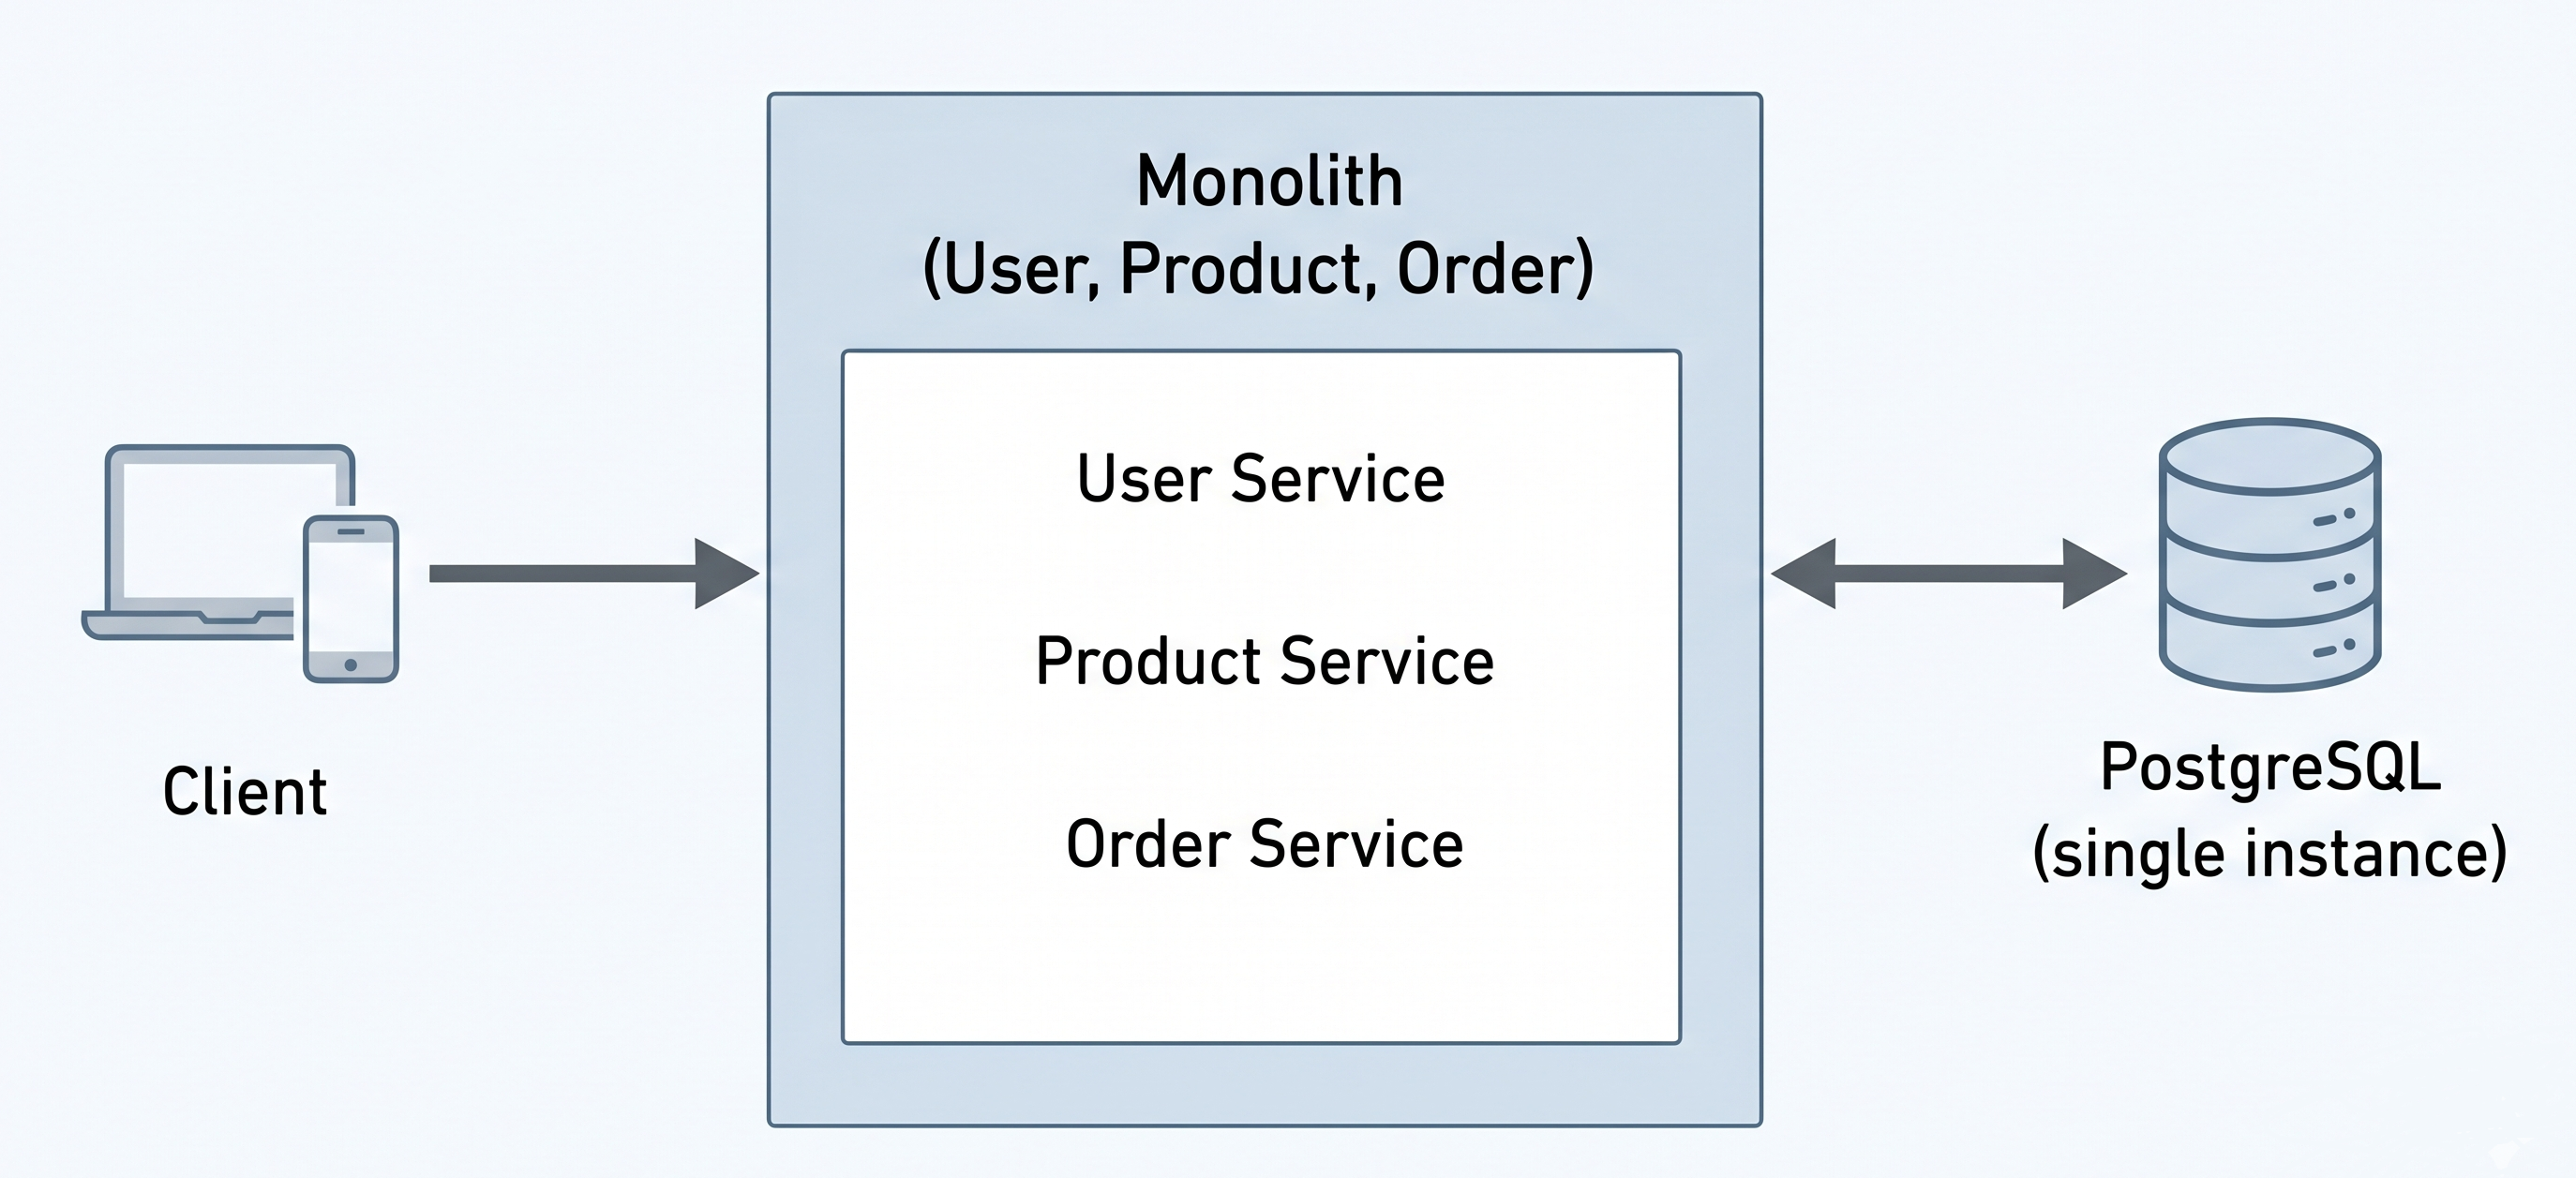
\includegraphics[width=\textwidth]{arch_monolith.png}
	\caption{Monolithic architecture used in the benchmark setup.}
	\label{fig-arch-monolith}
\end{figure}

\begin{figure}[ht]
	\centering
	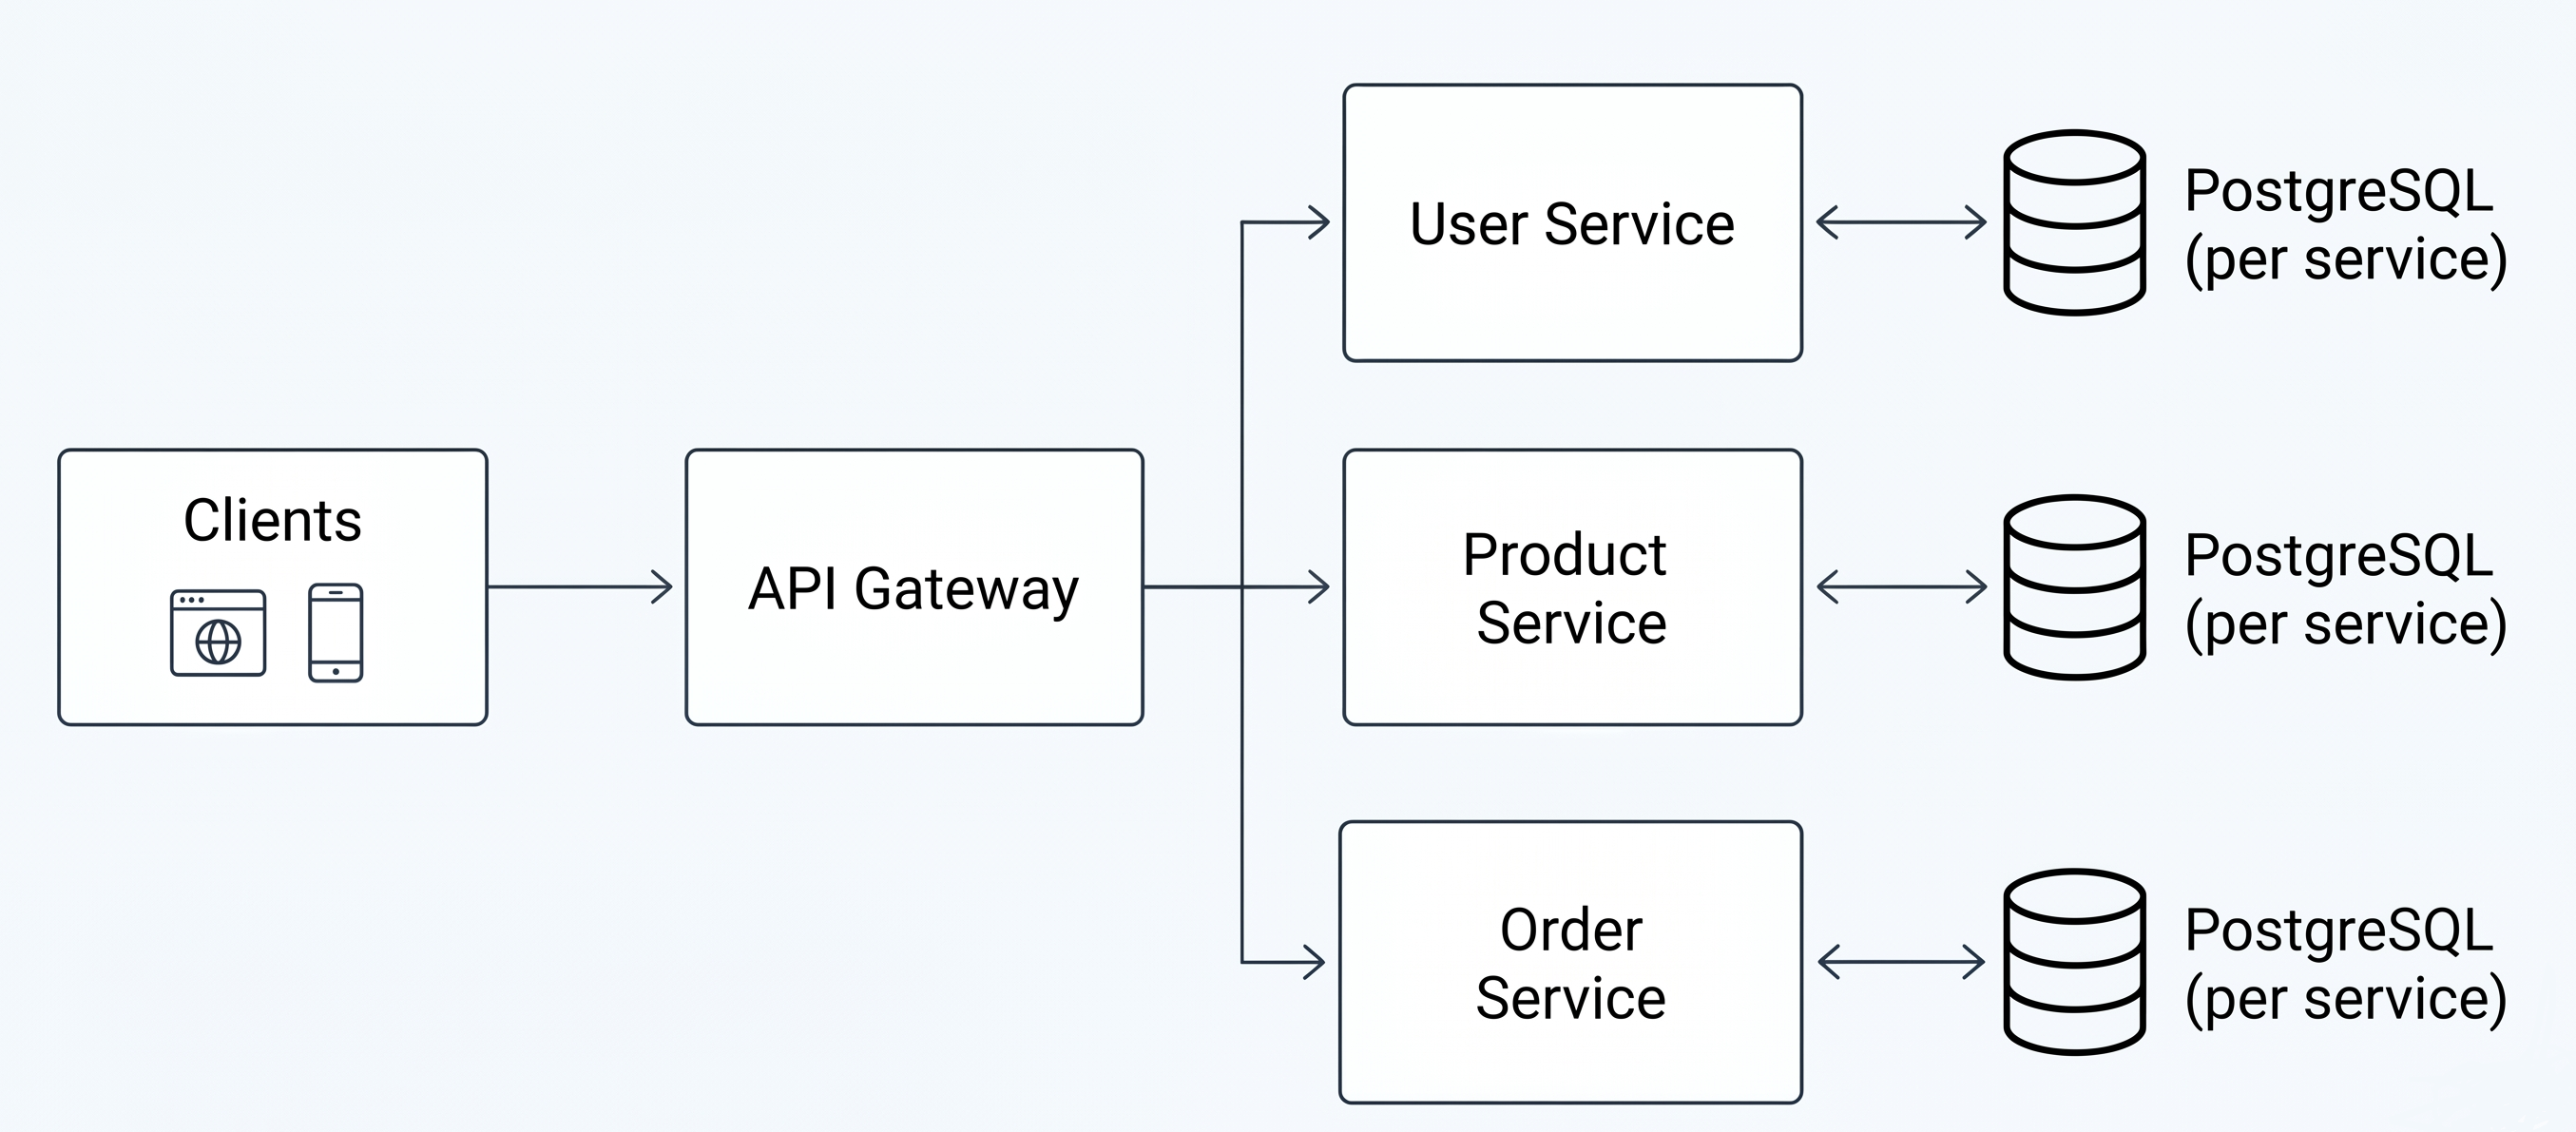
\includegraphics[width=\textwidth]{arch_micro.png}
	\caption{Microservices architecture used in the benchmark setup.}
	\label{fig-arch-microservices}
\end{figure}

To preserve fairness, both deployments use the same dataset and comparable total CPU and memory limits at the application tier.

\subsection{Execution Environment}\label{sec-execution-environment}

The fact that both architectures were running on the same physical hardware (the authors' laptop) due to the costs associated with renting out separate cloud resources is identified as the major limitation of this study. That being said, the limitations of this study are clearly outlined: while the two architectures could not be run simultaneously (they ran sequentially), because they both were executing on the same hardware, any observed throughput differences between them include whatever resource competition issues arise from the operating system when sequential runs occur. To mitigate this issue, the authors implemented several measures including creating resource constraints for each container within the Docker Compose environment in which each individual run was executed, and resetting each run's data before each execution; additionally, the authors applied a 'cooldown' period between runs. Each run was executed in its own isolated Docker container, and it required approximately nine hours to complete the entire experiment. Despite these considerations, the absolute values of throughput should be viewed in light of these conditions. More reliable insights can be found in how each architecture performs relatively under the same levels of introduced stress compared to their respective baselines (i.e., their performance under normal conditions).

Hardware and platform details are as follows: a 12th Gen Intel Core i5-1235U (10 physical cores, 12 logical threads), 24 GB RAM (approximately 23 GiB visible to the OS), running Linux x86\_64.

\subsection{Workload Model}

\begin{table}[ht]
	\caption{Workload model used in the benchmark.}
	\centering
	\begin{tabular}{l c}
		\toprule
		Operation class & Share \\
		\midrule
		Product reads   & 50\%  \\
		User reads      & 30\%  \\
		Order creation  & 20\%  \\
		\bottomrule
	\end{tabular}
	\label{workload_model}
\end{table}

Table \ref{workload_model} illustrates the Workload Model used to test the monolithic and microservices architectures. It shows a read-heavy profile designed to simulate e-commerce catalog traffic, which was generated using the Apache JMeter tool \cite{jmeter}. The workload mix was designed to reflect a read-heavy e-commerce traffic profile, where catalog browsing significantly outnumbers purchases. The 50/30/20 split product reads, user reads, and order creation respectively approximates the general shape reported in industry analyses of web retail traffic, where checkout events typically represent 15--25\% of session activity while product browsing dominates. Product reads were weighted highest because the product service is the shared dependency across all three stress scenarios: it is the target of fault injection, the source of latency injection, and a consumer of the shared connection pool. Concentrating load on this path ensures that injected failures and delays have a clear propagation path to measure, rather than being diluted across endpoints that do not interact.

\subsection{Experimental Scenarios}

In order to test and measure the ability of the monolithic and microservices architectural styles to be resilient under faults and delays; this study is based on four sets of experimental scenarios. The degree of complexity within these experiment scenarios range from a baseline condition to high levels of data tier contention as shown in Table~\ref{experimental_scenarios}.

\begin{table}[ht]
	\caption{Experimental scenarios and configuration summaries.}
	\centering
	\begin{tabular}{p{0.28\textwidth} p{0.18\textwidth} p{0.46\textwidth}}
		\toprule
		Scenario                       & Intent                  & Configuration summary                                                        \\
		\midrule
		Baseline                       & Reference               & No injected faults or delays; default pool settings                          \\
		Deterministic endpoint failure & Failure propagation     & Product-read failures injected for a fixed ID set                            \\
		Latency injection              & Performance degradation & Fixed delay injected on product-read path                                    \\
		Pool exhaustion sweep          & Data-tier contention    & Connection pool sizes swept across \texttt{2, 5, 10} with fixed request load \\
		\bottomrule
	\end{tabular}
	\label{experimental_scenarios}
\end{table}

The logic for implementing fault and latency injection in both architectural types (the product read path) was identical. These injections were also controlled via run-time properties which include \texttt{chaos.enabled},\texttt{chaos.mode},\texttt{chaos.fault.ids}, and \texttt{chaos.latency.ms}\cite{chaos_engineering_principles}. A request will fail only when it requests a product id that has been identified as one of the ids contained within a predefined static list. This allows for the avoidance of random sample noise, thereby improving the reproducibility of results between multiple runs of each architecture.

\subsection{Connection Pool Stress Protocol}

Stress testing pools involves varying the maximum number of pools while maintaining a constant number of concurrent requests. Therefore, it allows us to isolate resource issues related to limited database handles. This paper test three different pool sizes (\texttt{2, 5, 10}), it executes multiple repeats of the same pool size and analyze them independently for both architectures. Each run resets all environmental settings to prevent any state carried over and sets the connection timeout to \texttt{2000 ms} during our pool-stress tests; therefore if a connection times out that will be counted as an error against the request.

This research uses the following definitions when interpreting pool and connection limits based upon pool configuration behavior and the database's own limit on connections. \cite{hikaricp,postgres_max_connections}

\subsection{Statistics and Metrics Analysis }

The focus of this study was measuring the following metrics: throughput (number of requests per second), latency percentiles (P50, P95, P99), error rates and error counts, and time series plots for throughput and tail latencies.

All results for each scenario were measured at the individual run level and aggregated at the architectural level. The analysis pipeline calculates the mean, standard deviation, and 95\% confidence interval for each metric, and finally provides delta values between architectures as well as degradation relative to base line whenever base line data is available.

\subsection{Run Execution and Reproduction}

All runs are executed separately using Docker Compose \cite{docker_compose}. The execution process first initializes the architecture and waits for health check completion, initiates Jmeter workload execution, stores raw .jtl output and html report files after run completion, removes all containers/volumes, and adds a delay prior to executing subsequent run(s) as a cooldown period.

Results are stored along with timestamps for the respective scenario. Metadata associated with each run is preserved, as well as raw measurements and processed summaries for each aggregate (run, scenario) level. Reproductive procedures employed here utilize best practices developed for reproducibility in computational science workflows \cite{peng_reproducible_research}.

\section{Experimental Results}\label{sec-results}

This section reports the final experimental campaign. Scenario-level statistics are summarized with repeated-run aggregates, confidence intervals, and architecture deltas. Unless noted otherwise, numeric scores in this section come from the generated summary tables \cite{scenario_architecture_stats_table,architecture_delta_by_scenario_table,pool_sweep_summary_table}.

\begin{table}[ht]
	\caption{Scenario-level performance summary by architecture.}
	\label{tab-scenario-performance-summary}
	\centering
	\begin{tabular}{l l r r r}
		\toprule
		Scenario              & Architecture  & Throughput (req/s) & P95 (ms) & Error rate (\%) \\
		\midrule
		Baseline              & Monolith      & 3420.1             & 199.0    & 0.00            \\
		Baseline              & Microservices & 1291.1             & 493.7    & 0.77            \\
		Deterministic fault   & Monolith      & 3326.4             & 203.7    & 9.33            \\
		Deterministic fault   & Microservices & 1144.6             & 732.3    & 10.78           \\
		Latency injection     & Monolith      & 107.5              & 3175.0   & 41.18           \\
		Latency injection     & Microservices & 198.7              & 2450.9   & 47.44           \\
		Pool exhaustion (agg) & Monolith      & 3171.9             & 157.8    & 0.00            \\
		Pool exhaustion (agg) & Microservices & 1305.2             & 479.9    & 0.28            \\
		\bottomrule
	\end{tabular}
\end{table}

Table~\ref{tab-scenario-performance-summary} shows that the two architectures respond to stress very differently. Under baseline and pool conditions, the monolith maintains a throughput advantage of roughly 2.6$\times$ and a P95 latency advantage of roughly 2.5$\times$. Under latency injection, that advantage reverses in one dimension: the monolith's throughput collapses more severely (107.5 vs 198.7 req/s) while its tail latency grows larger (3175 vs 2450 ms), even though microservices accumulates a higher overall error rate. Neither architecture dominates across all scenarios the pattern depends on which stress dimension you measure.

Cross-scenario aggregates provide a compact view of architecture-level differences across baseline, failure, latency, and pool-stress conditions, as shown in Figures~\ref{fig-scenario-comparison} and \ref{fig-scenario-boxplots}.

\begin{figure}[ht]
	\centering
	
\includegraphics[width=\textwidth]{scenario_comparison_ci.png}
	\caption{Cross-scenario comparison of throughput, P95 latency, and error rate (mean with 95\% confidence intervals).}
	\label{fig-scenario-comparison}
\end{figure}

\begin{figure}[ht]
	\centering
	
\includegraphics[width=\textwidth]{scenario_boxplots.png}
	\caption{Run-level metric distributions by scenario and architecture.}
	\label{fig-scenario-boxplots}
\end{figure}

\subsection{Baseline Performance}

Under baseline load, the monolith achieved substantially higher throughput and lower tail latency than the microservices deployment.
Monolith mean throughput was \texttt{3420.1 req/s} versus \texttt{1291.1 req/s} for microservices, a throughput delta (micro vs mono) of \texttt{-62.25\%}.
Monolith mean P95 was \texttt{199.0 ms}, while microservices mean P95 was \texttt{493.7 ms}.

These differences are consistent across repeated runs. Throughput confidence intervals are narrow for both architectures, while microservices show wider P95 uncertainty. Baseline endpoint behavior and throughput stability are shown in Figures~\ref{fig-baseline-endpoint-comparison} and \ref{fig-baseline-throughput-over-time}.

\begin{figure}[ht]
	\centering
	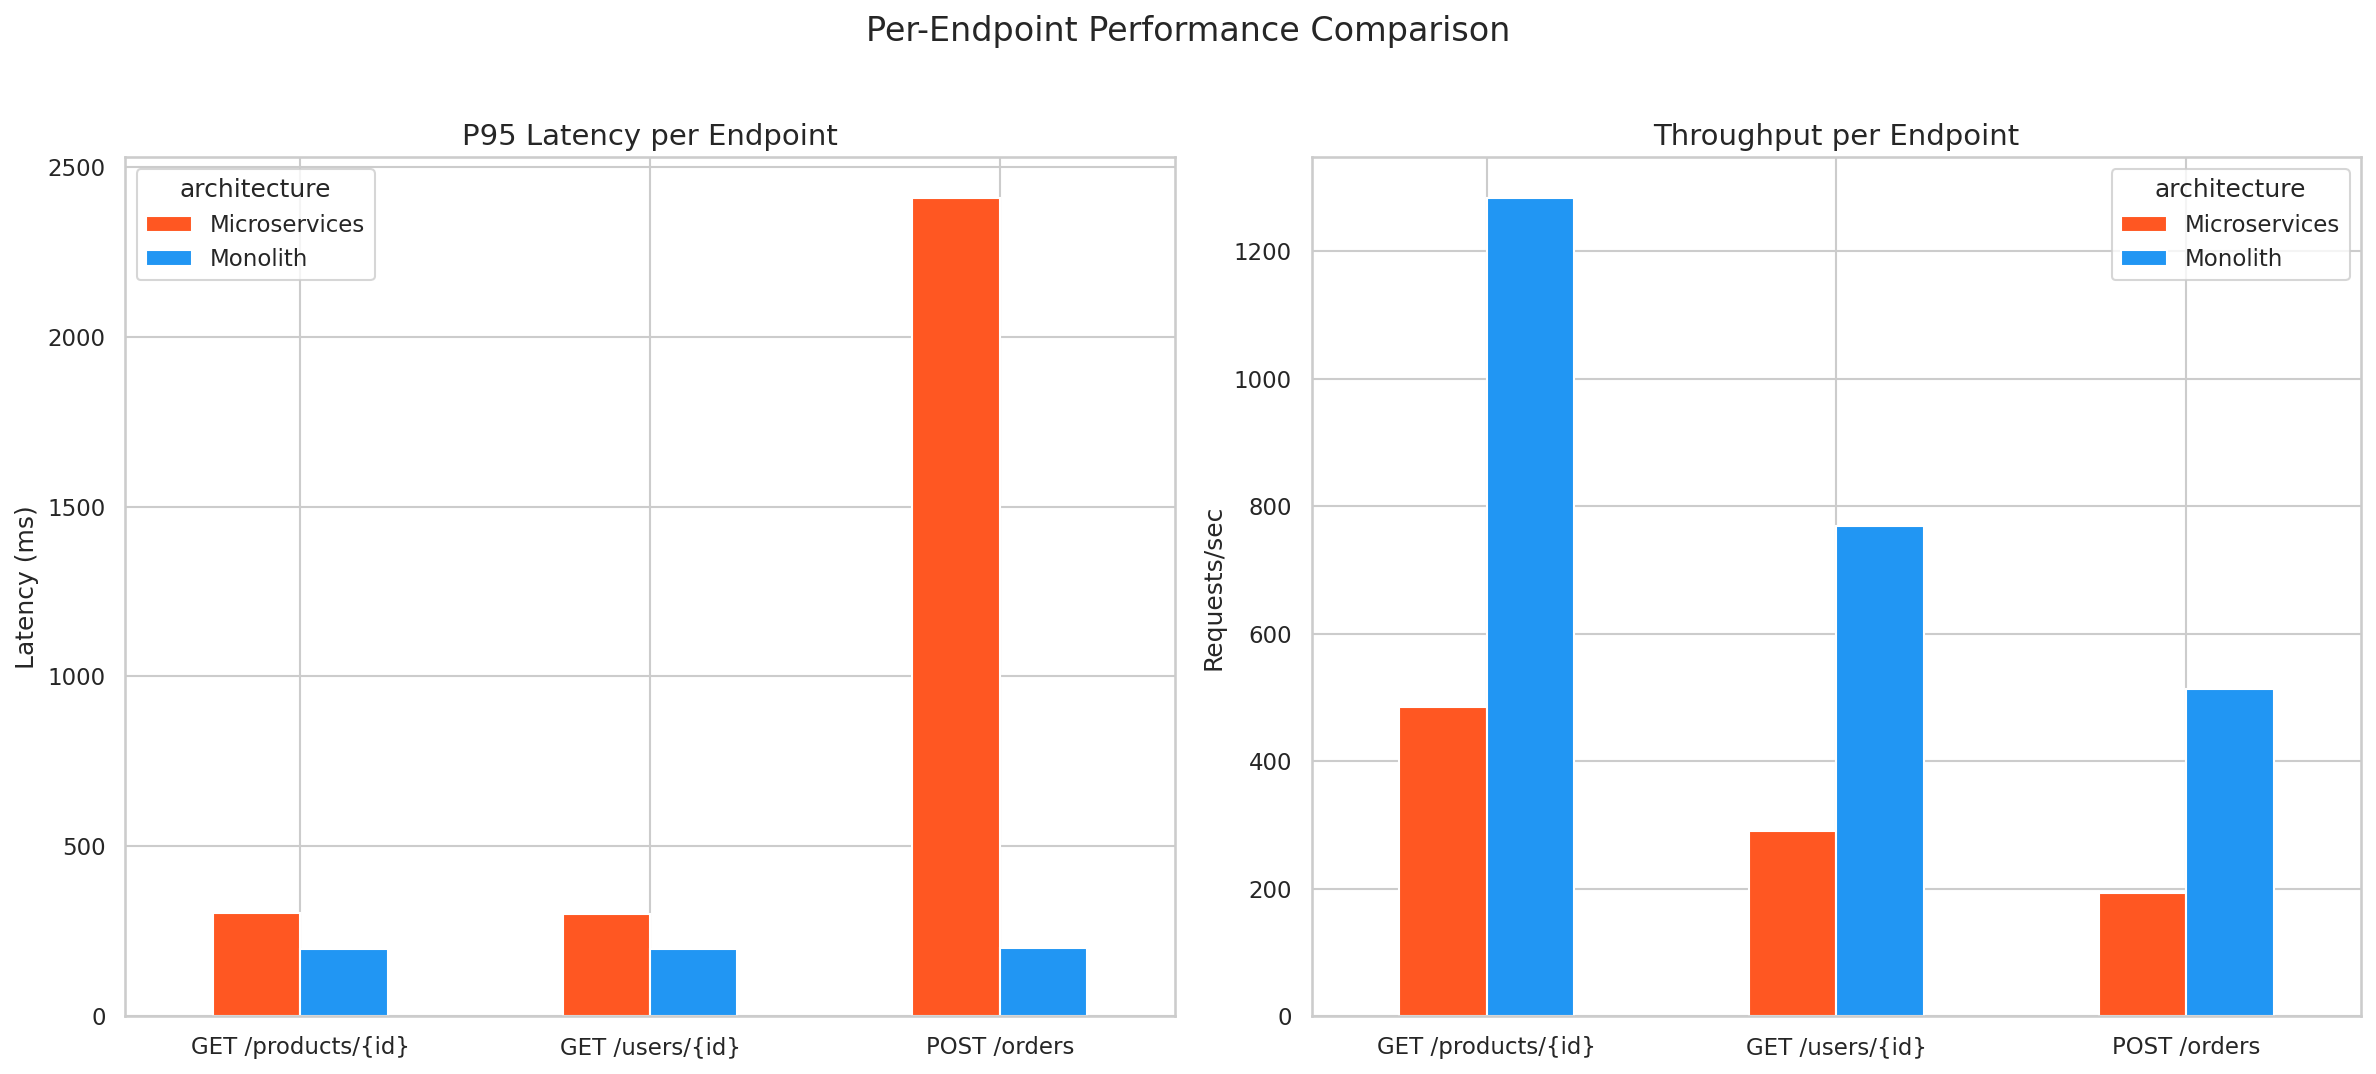
\includegraphics[width=\textwidth]{per_endpoint_comparison.png}
	\caption{Baseline endpoint comparison between architectures (throughput and latency characteristics by API path) confirming that the performance gap is consistent across all three endpoints, not isolated to a single path.}
	\label{fig-baseline-endpoint-comparison}
\end{figure}

\begin{figure}[ht]
	\centering
	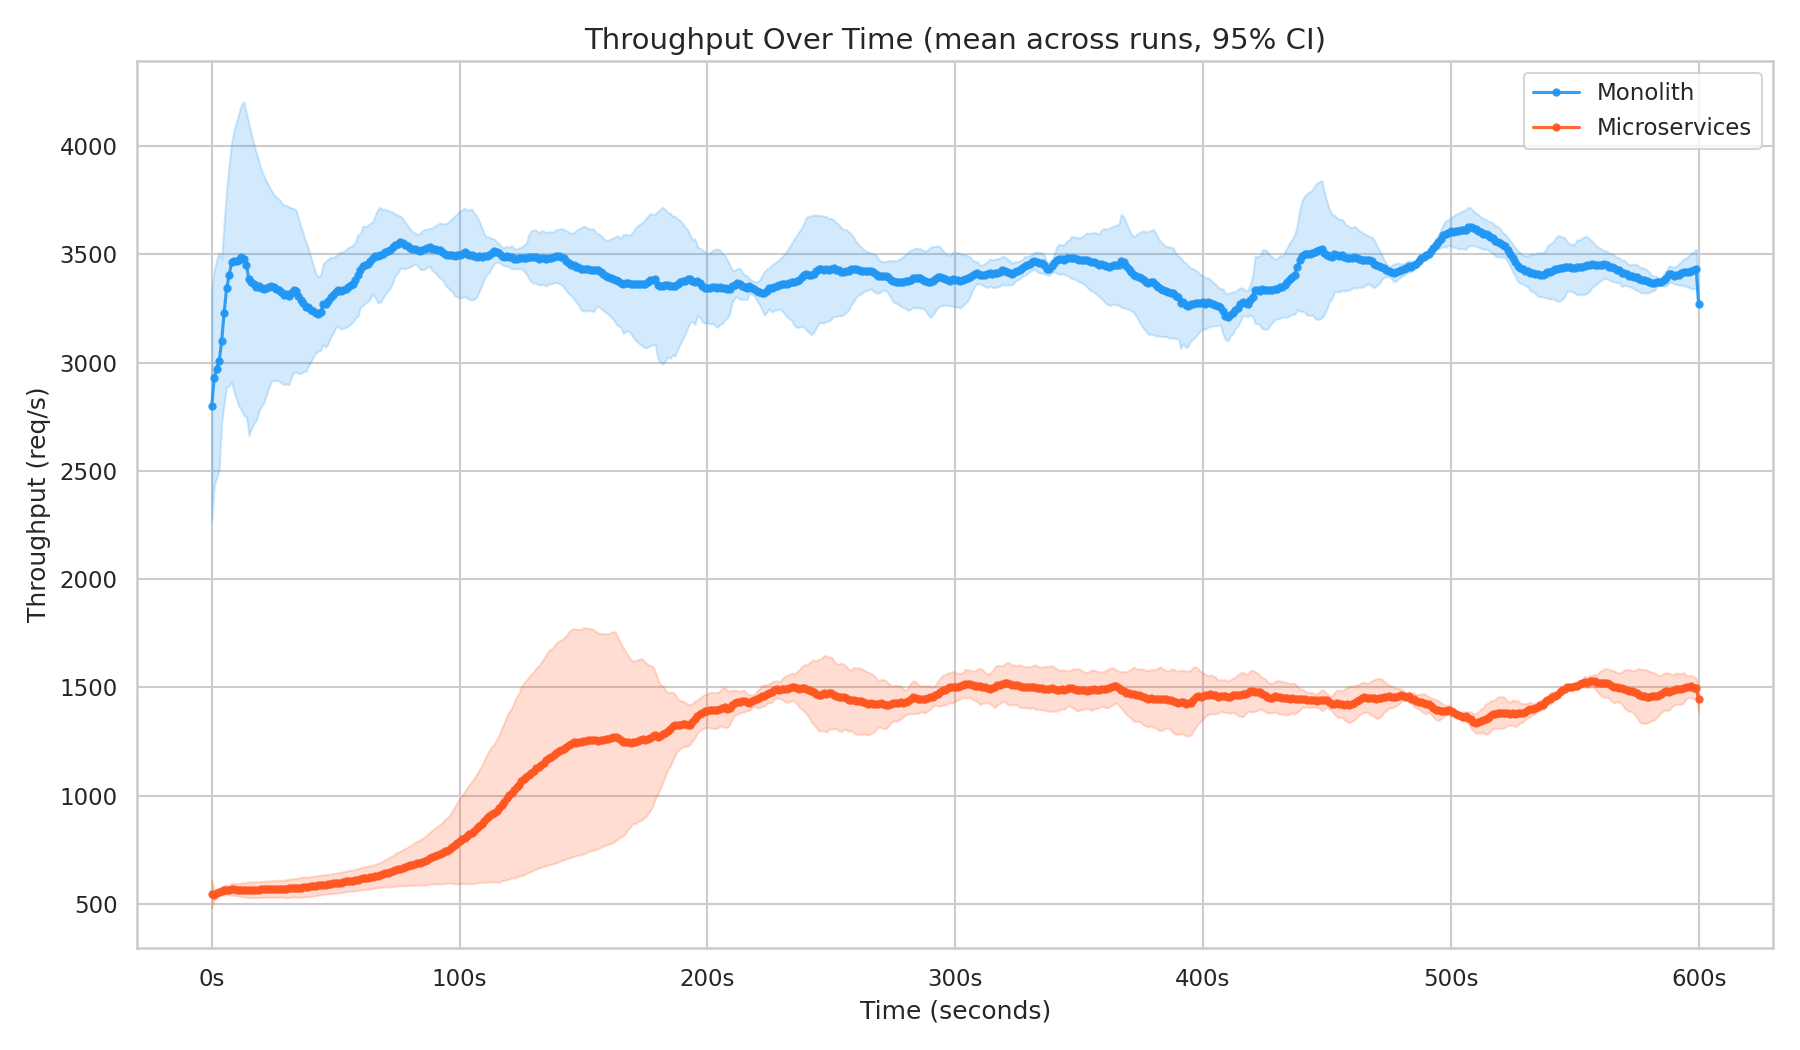
\includegraphics[width=\textwidth]{throughput_over_time.png}
	\caption{Baseline throughput over normalized run time (mean across runs) showing that the performance gap is not a warm-up artefact but a persistent steady-state difference.}
	\label{fig-baseline-throughput-over-time}
\end{figure}

\subsection{Deterministic Endpoint Failure}

Deterministic fault injection used the fixed ID set \texttt{3, 7, 11, 12}, which represents \texttt{4/30 = 13.33\%} of product IDs. The \texttt{GET /products/\{id\}} error rate was \texttt{13.33\%} (monolith) vs \texttt{13.36\%} (microservices), while the scenario-level error rate was \texttt{9.33\%} (monolith) vs \texttt{10.78\%} (microservices). Throughput was \texttt{3326.4 req/s} (monolith) vs \texttt{1144.6 req/s} (microservices), and P95 latency was \texttt{203.7 ms} (monolith) vs \texttt{732.3 ms} (microservices).

Endpoint-level decomposition shows stronger downstream amplification in microservices order creation, as illustrated in Figure~\ref{fig-fault-per-endpoint-error-rate}.

\begin{figure}[ht]
	\centering
	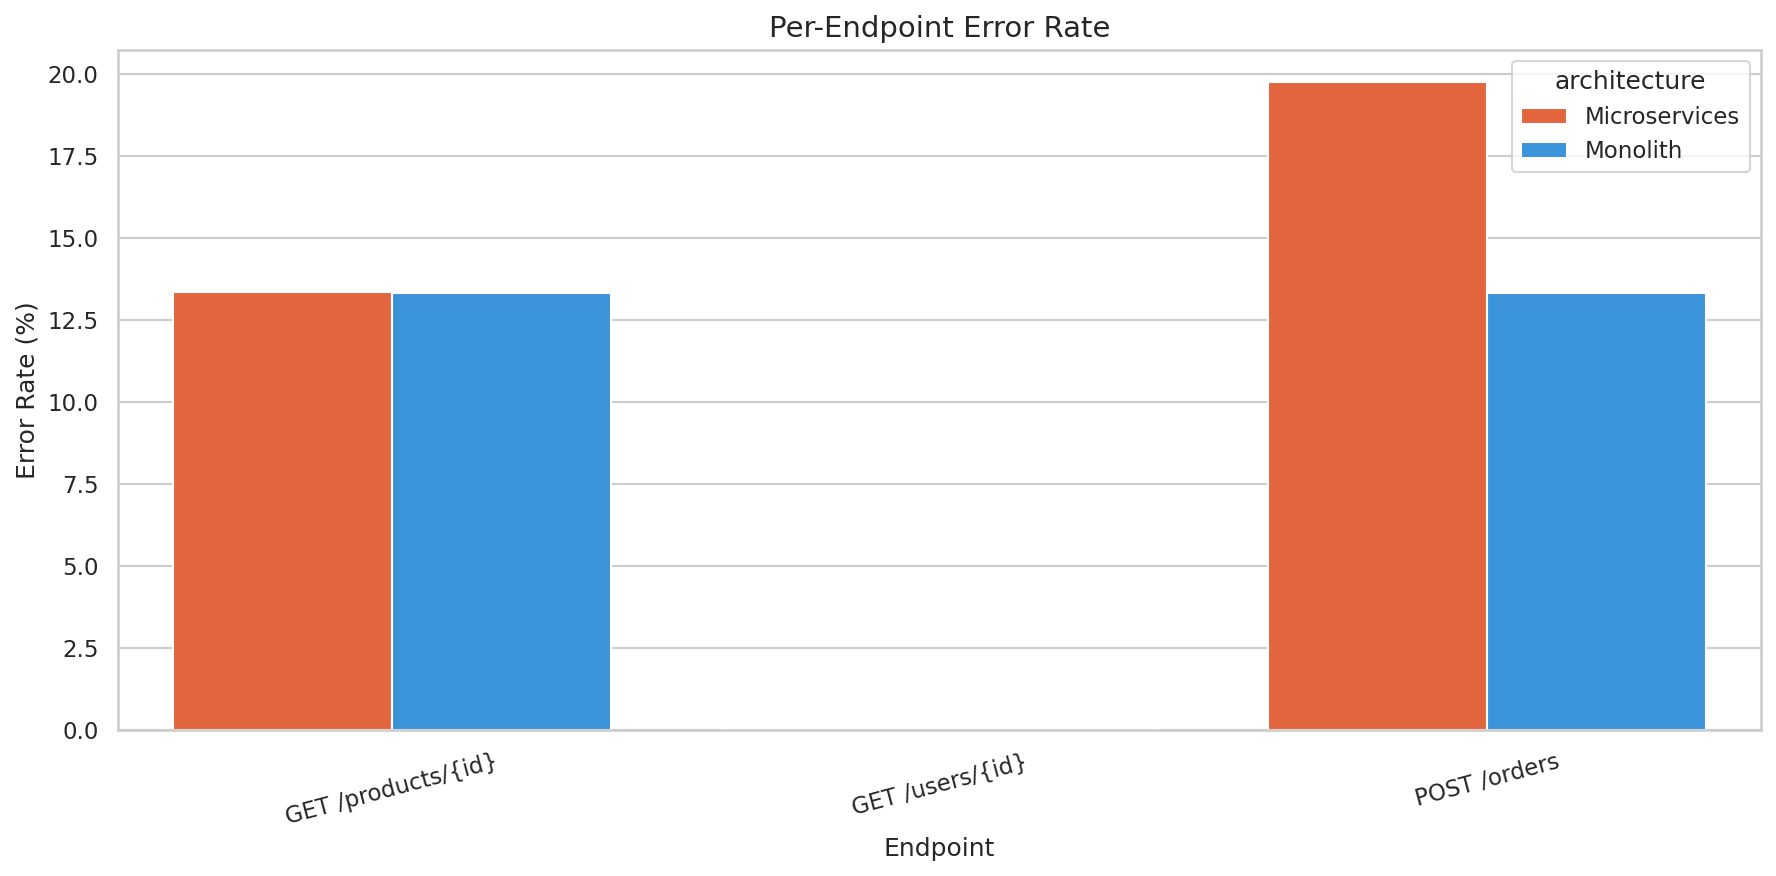
\includegraphics[width=0.85\textwidth]{fault_per_endpoint_error_rate.png}
	\caption{While product-endpoint error rates are nearly identical between architectures ($\approx$13.3\%), the microservices POST /orders endpoint shows significantly higher failure evidence that synchronous inter-service dependency amplifies upstream faults into composite operations.}
	\label{fig-fault-per-endpoint-error-rate}
\end{figure}

\subsection{Latency Injection}

Latency injection produced the strongest degradation in both architectures, with severe tail-latency growth and error-rate increases. The monolith measured \texttt{107.5 req/s}, \texttt{P95 3175.0 ms}, and \texttt{41.18\% errors}, while microservices measured \texttt{198.7 req/s}, \texttt{P95 2450.9 ms}, and \texttt{47.44\% errors}.

Although throughput collapsed in both systems under this stress, aggregate P95 latency was higher for the monolith, while microservices showed higher overall error and stronger end-to-end failure in order processing. Endpoint-level errors are shown in Figure~\ref{fig-latency-per-endpoint-error-rate}, and temporal endpoint latency behavior is shown in Figure~\ref{fig-latency-endpoint-over-time}.

\begin{figure}[ht]
	\centering
	
\includegraphics[width=0.85\textwidth]{latency_per_endpoint_error_rate.png}
	\caption{Per-endpoint error rates under latency injection showing that injected latency on the product path cascades into total order-creation failure when services are synchronously chained.}
	\label{fig-latency-per-endpoint-error-rate}
\end{figure}

\begin{figure}[ht]
	\centering
	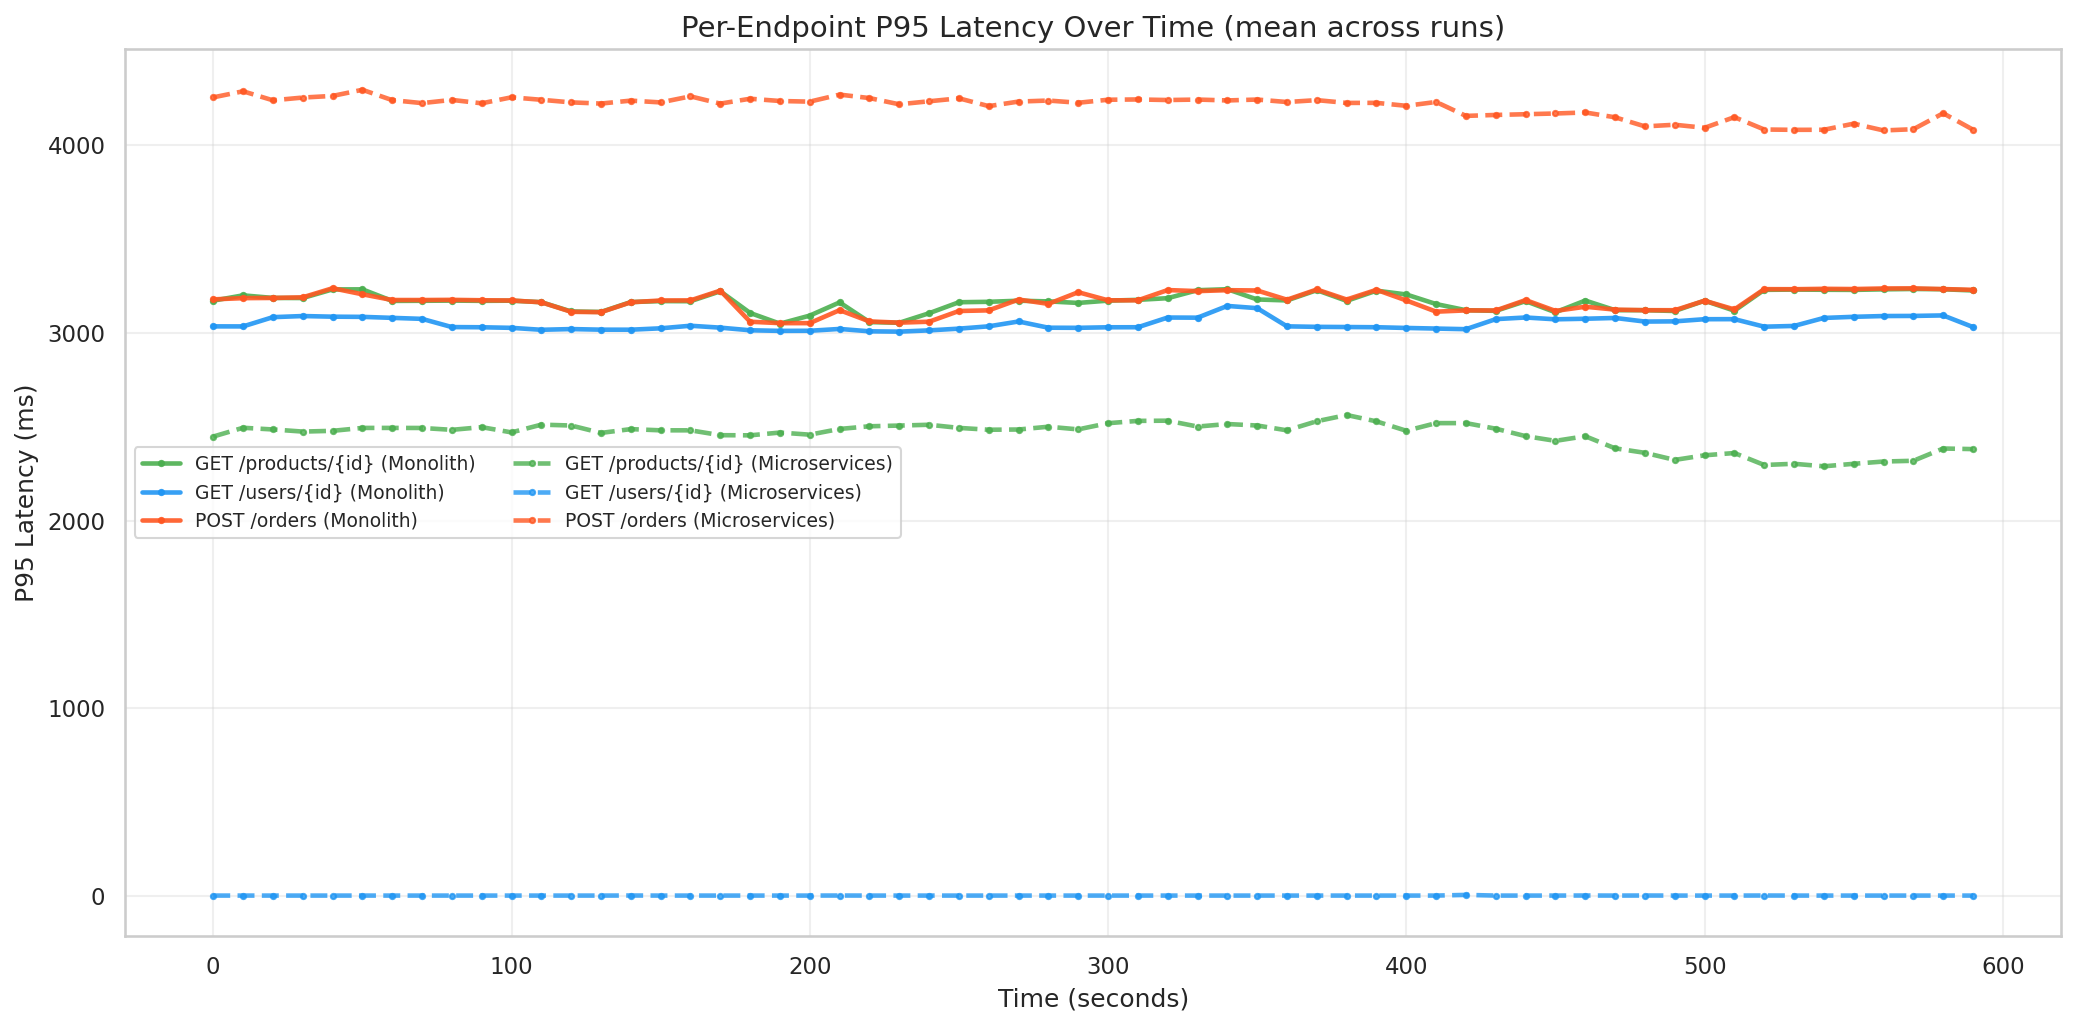
\includegraphics[width=\textwidth]{endpoint_latency_over_time.png}
	\caption{Latency injection time-series by endpoint and architecture (run-averaged) indicating that tail latency compounds along the service chain rather than recovering over time.}
	\label{fig-latency-endpoint-over-time}
\end{figure}

\subsection{Pool Exhaustion Sweep}\label{sec-pool-exhaustion-sweep}

Pool-size sweeps reveal architecture-dependent contention behavior. Monolith throughput dropped sharply at pool size \texttt{2} compared with \texttt{5} and \texttt{10}, while the microservices architecture showed its highest throughput at pool size \texttt{2} and its highest observed error rate at pool size \texttt{10}.

Given the fixed \texttt{2000 ms} timeout, queueing pressure can convert into timeout-driven failures; however, the observed error response is non-monotonic and architecture-specific rather than a simple inverse function of pool size.

This pattern suggests that connection-pool tuning should be architecture-specific rather than transferred directly between deployment styles, consistent with the sweep trends in Figure~\ref{fig-pool-sweep-metrics}.

\begin{figure}[ht]
	\centering
	
\includegraphics[width=\textwidth]{pool_sweep_metrics.png}
	\caption{Pool-size response is non-monotonic and architecture-specific. The monolith loses throughput sharply below pool size 5, while microservices peaks at size 2 and accumulates errors at size 10 indicating that connection governance strategies cannot be shared between deployment styles.}
	\label{fig-pool-sweep-metrics}
\end{figure}

\section{Discussion}\label{sec-discussion}

The results support three main observations.

This research found the baseline gap in throughput much greater than anticipated: 3420 reqs/sec vs. 1291 reqs/sec. While we expected the monolith would be faster, it wasn't by a factor of 2.6$\times$; part of that gap will almost certainly be amplified by shared-host resource contention, as described in Section~\ref{sec-execution-environment}, however, even discounting that, the difference in P95 latency (199 ms vs. 493 ms) is very difficult to rationalize by resource competition alone with a 2.5$\times$ difference in tail latency for a straightforward read operation. It seems the most plausible reason for the large difference in latency is due to serialized wait times introduced by the API Gateway and HTTP hops between services that compound at the tail end of the distribution, similar to what Dean and Barroso have described as the "straggler" problem in large-scale distributed service graphs. As such, the gap has significant implications for teams working under constraint hardware resources - the microservice implementation is currently consuming about half of available performance before load is added \cite{dean_tail_at_scale,deathstarbench}.

The failure injection results reveal a surprisingly consistent pattern across architectures: product-endpoint error rates are nearly identical (13.33\% for monolithic architecture vs 13.36\%) yet, scenario-level error rates diverge by 9.33\% for the monolithic architecture and by 10.78\% for microservices. Although this 1.45 percentage point difference may seem small, it is the cost of synchronous inter-service calls amplifying the failure. A single failed product lookup in the monolith will fail only for that request and no further. Conversely, the same failure will propagate into the order service which requires successful validation of the product before completing. Since circuit breaker or retry logic were not implemented in this experiment to measure purely the behavior where failure was propagated through the services (as well as because adding those controls would have made the implementations less comparable), the implication is that while micro-services do not necessarily need explicit resilience patterns at the request level (they just move where the failure lands \cite{google_sre}), they are not more fault-tolerant without them.

The findings from the pool sweep were the most surprising part of the overall findings. It was anticipated that there would be an obvious correlation between the size of the pool and how many contentions occur, thus determining how well each service performs. However, the data showed that when using two services (pool size = 2), the throughput for microservices was best. Then as you continued to add services to the pool and increase its size, throughput began to degrade. There is speculation about what could be happening here; one possible reason is that when using a pool size of 2, the microservice gateway will aggressively queue up all the requests received by it and process them in small groups. Processing these small groupings may help lower the amount of overhead created due to partial transaction processing and context switching. When the pool size increases, more concurrent requests are sent to the database at once. In addition, the overhead associated with managing all of these connections appears to exceed the benefits derived from this concurrency at least while operating within the confines of a single host's resource constraints. This is purely speculative and it is also the type of finding that should warrant further experimentation on dedicated hardware. At least it can be concluded with certainty that if you take a configuration of your connection pooling from your monolithic deployment, do not apply it to your microservices deployment and expect to get similar results \cite{hikaricp,postgres_max_connections}.

From an engineering perspective, these findings suggest that microservices require stricter reliability controls (timeouts, retry discipline, backpressure, and pool governance) to prevent localized degradation from becoming user-visible failure in composite paths \cite{resilience_patterns,google_sre}.

\subsection{Threats to Validity}

The primary threats to validity of this research include the issues of internal validity; the study focused solely on one domain model, and therefore only reflects the performance of that single model. In addition, only one workload-mix was tested, and thus only reflects how well the chosen mix performs under those conditions. And finally, the study utilized a singular implementation-stack, and therefore can provide no insight into how well either system would perform using alternative stacks. Although deterministic injection allows for greater reproducibility, it also represents a worst-case-scenario when compared to random production-failure distributions. The construct-validity of this research is also limited in its ability to measure orchestration-driven restart-resilience through the use of endpoint-level fault-injection. The largest limitation of this research - from a resource perspective - is due to the fact that both systems were deployed onto the same physical server. Therefore, all services (monolith or microservices) were competing for the same underlying CPU and memory resources creating implicit contention that could not be completely removed. Three methods were used to mitigate against this: apply Docker resource-limits to capping both services' CPU and memory allocations, reset the container-state after every run to ensure the warm-cache advantage was avoided, and isolate runs completely with a cool-down-period prior to starting the subsequent run. Nevertheless, these controls will never eliminate OS-scheduling impacts entirely. As such, readers should treat absolute-throughput-numbers as indicative rather than definitive and give a larger amount of credence towards the degradation-relativerobase-analysis since the relative-comparison-within-each-architecture is impacted less-by-the-shared-server-issue compared-to-cross-architecture comparisons.

\subsection{Reproducibility Artifact}

Source code and experiment automation are available at:

the project repository:
Source code and experiment automation are publicly available at \cite{repo_artifact}.

\subsection{Results Conclusion}

Table ~\ref{tab-results-summary} presents the major performance outcomes of the various benchmarks.
The baseline results illustrate that a monolithic system provided far greater throughput and less extreme tail latency compared to a micro-services based architecture under equivalent workloads and resources.
When endpoint failures were deterministically simulated in each case, as expected both architectures suffered from increased error rates; however, because of dependency chaining, the micro-services configuration exhibited a larger growth in p95 latency (indicating how far failures propagated through the service chain).
Artificial delay caused the largest decline in performance for both configurations, severely limiting throughput and increasing error-rates as it would be expected to impact end-user experience.
In contrast to when endpoint failures occurred, the pool-exhaustion test demonstrated that although the monolithic design was relatively unaffected by the loss of connections in the pool, the micro-service configuration continued to exhibit elevated latency levels and a modest error-rate, further emphasizing the need to adjust connection pools on a per architecture basis.

\begin{table}[ht]
	\caption{Results summary across scenarios and architectures.}
	\label{tab-results-summary}
	\centering
	\begin{tabular}{l l r r r}
		\toprule
		\textbf{Scenario}   & \textbf{Architecture} & \textbf{Throughput} (req/s) & \textbf{P95} (ms) & \textbf{Error Rate} (\%) \\
		\midrule
		Baseline            & Monolith              & 3420.1                      & 199.0             & 0.00                     \\
		                    & Microservices         & 1291.1                      & 493.7             & 0.77                     \\
		Deterministic Fault & Monolith              & 3326.4                      & 203.7             & 9.33                     \\
		                    & Microservices         & 1144.6                      & 732.3             & 10.78                    \\
		Latency Injection   & Monolith              & 107.5                       & 3175.0            & 41.18                    \\
		                    & Microservices         & 198.7                       & 2450.9            & 47.44                    \\
		Pool Exhaustion     & Monolith              & 3171.9                      & 157.8             & 0.00                     \\
		                    & Microservices         & 1305.2                      & 479.9             & 0.28                     \\
		\bottomrule
	\end{tabular}
\end{table}

\section{Conclusion}\label{sec-conclusion}

The Monolith exhibited a consistently better-than-baseline efficiency relative to the Microservice under the load condition and resource constraint provided, with significantly better throughput and tail latency. However, when subjected to an injection of stress, the degradation pattern was different based upon architecture; whereas tail-latency inflation could potentially degrade faster within the Monolith due to its non-isolated structure (and potentially greater shared state), Microservices retained some level of isolation across disparate paths; however, they also exhibited the potential for significantly worse error amplification and order/path-based tail-latency degradation. In addition, as demonstrated through Pool-Stress tests, it is also apparent that there are significant differences in how architectural parameters need to be tuned based on the overall system architecture being utilized. There is no direct correlation between increasing the number of connections available via a pool and either improving throughput or reducing latency; nor does timeout-driven error behavior correlate with pool size changes in a monotonic manner. Therefore, both connection and timeout parameter values should be measured and validated for each individual system type (Monolithic vs. MicroService) instead of assuming those settings would be directly transferable from one deployment methodology to another.

These findings do not establish a universal winner. Monoliths remain strong for performance efficiency and lower operational overhead in this setting, while microservices retain organizational and deployment flexibility when supported by mature reliability controls. Architecture selection is therefore best treated as a workload- and operations-driven decision, guided by explicit performance targets, failure budgets, and reproducible benchmarking.

\section{Appendix}\label{sec-appendix}

Additional diagnostic visualizations are provided for transparency and replication support; distributional and run-level tail-latency variability views are shown in Figures~\ref{fig-appendix-latency-distribution} and \ref{fig-appendix-p95-boxplot}.

\begin{figure}[ht]
	\centering
	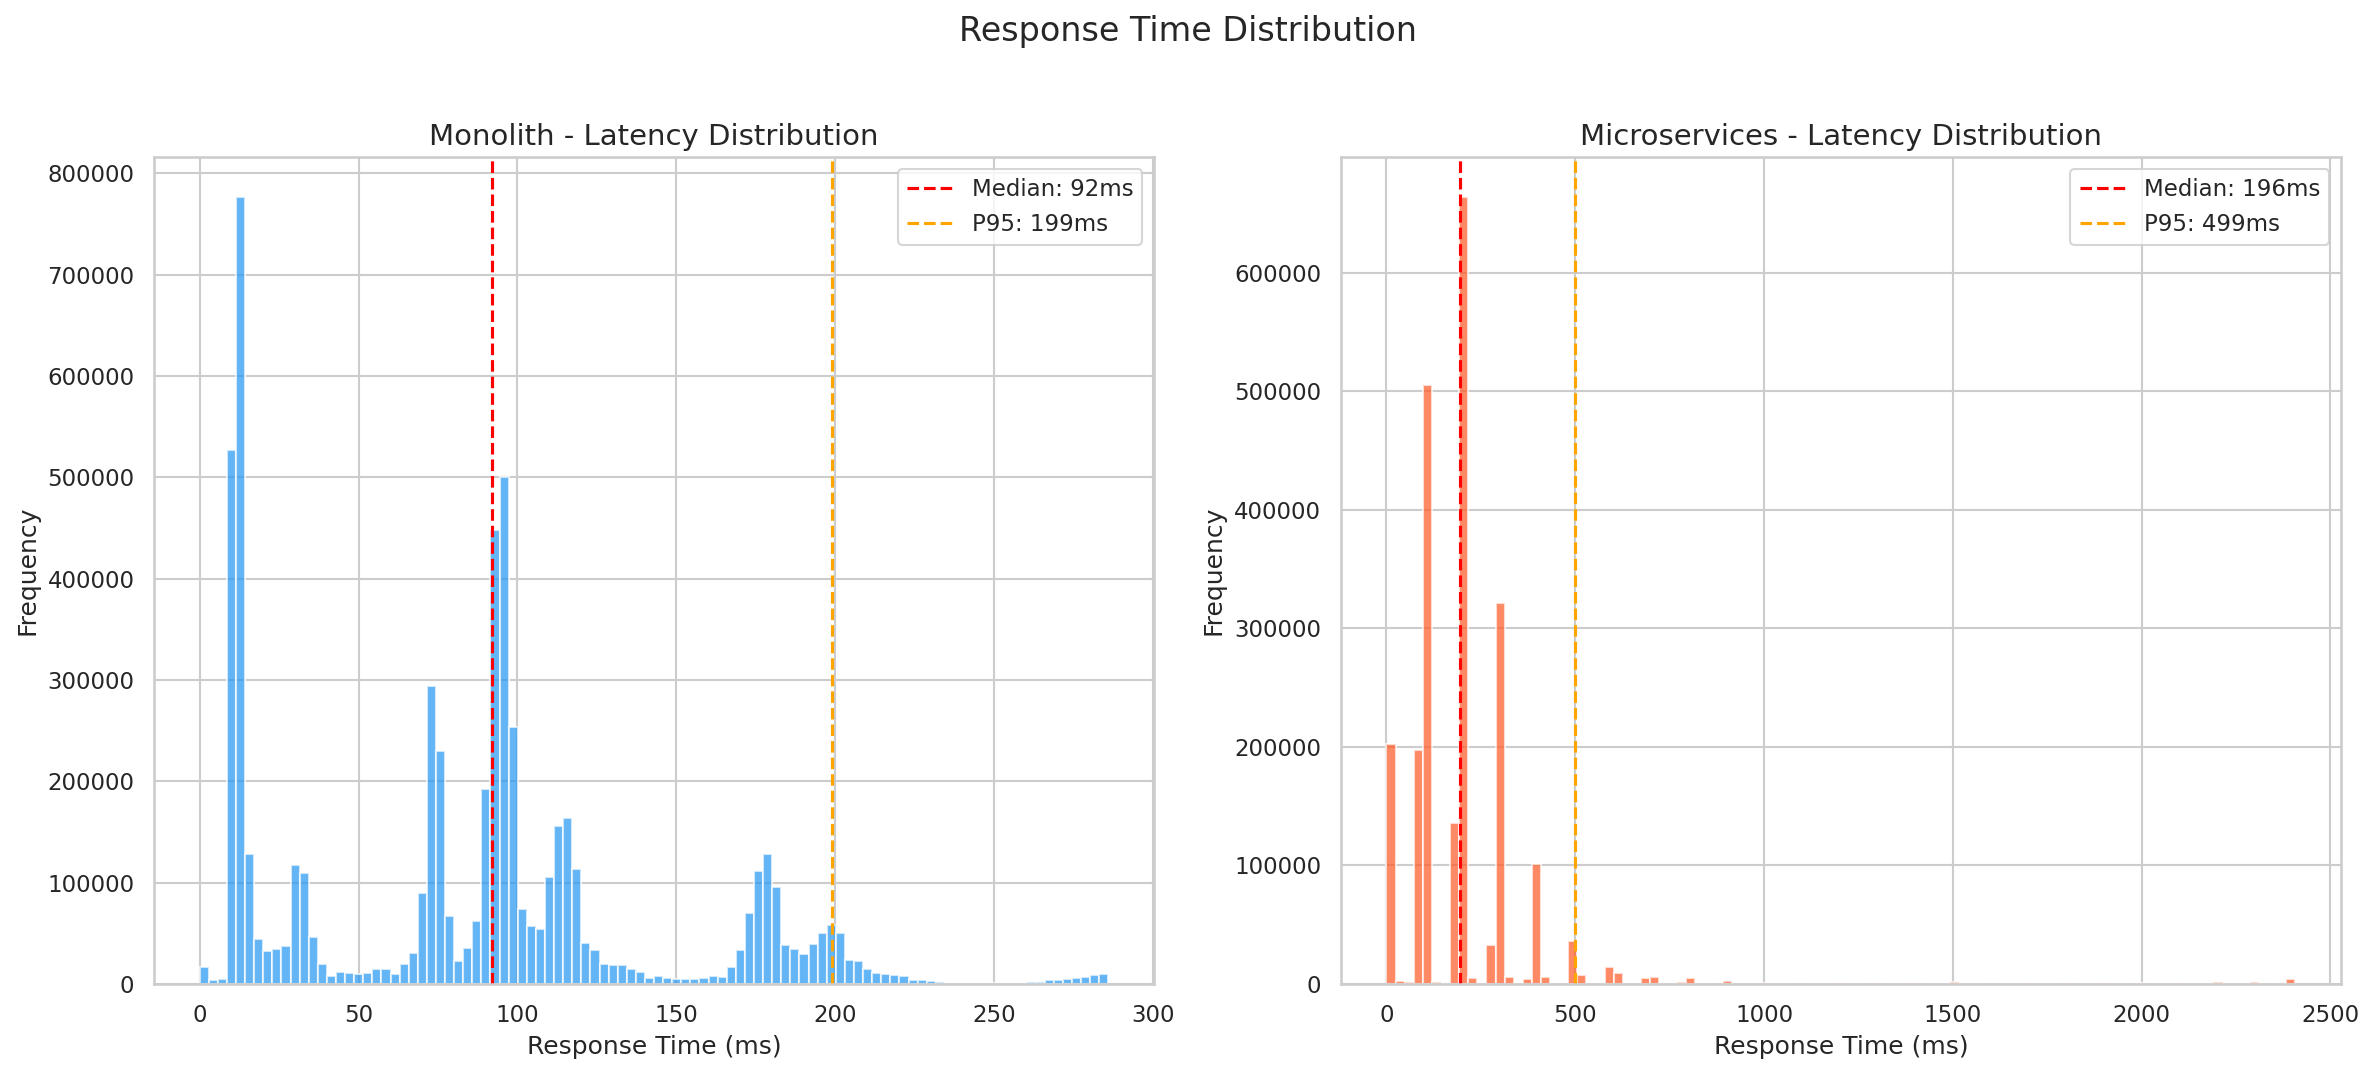
\includegraphics[width=\textwidth]{latency_distribution.png}
	\caption{Baseline latency distribution by architecture, the broader distribution means microservices users experience far more variability even under normal load.}
	\label{fig-appendix-latency-distribution}
\end{figure}

\begin{figure}[ht]
	\centering
	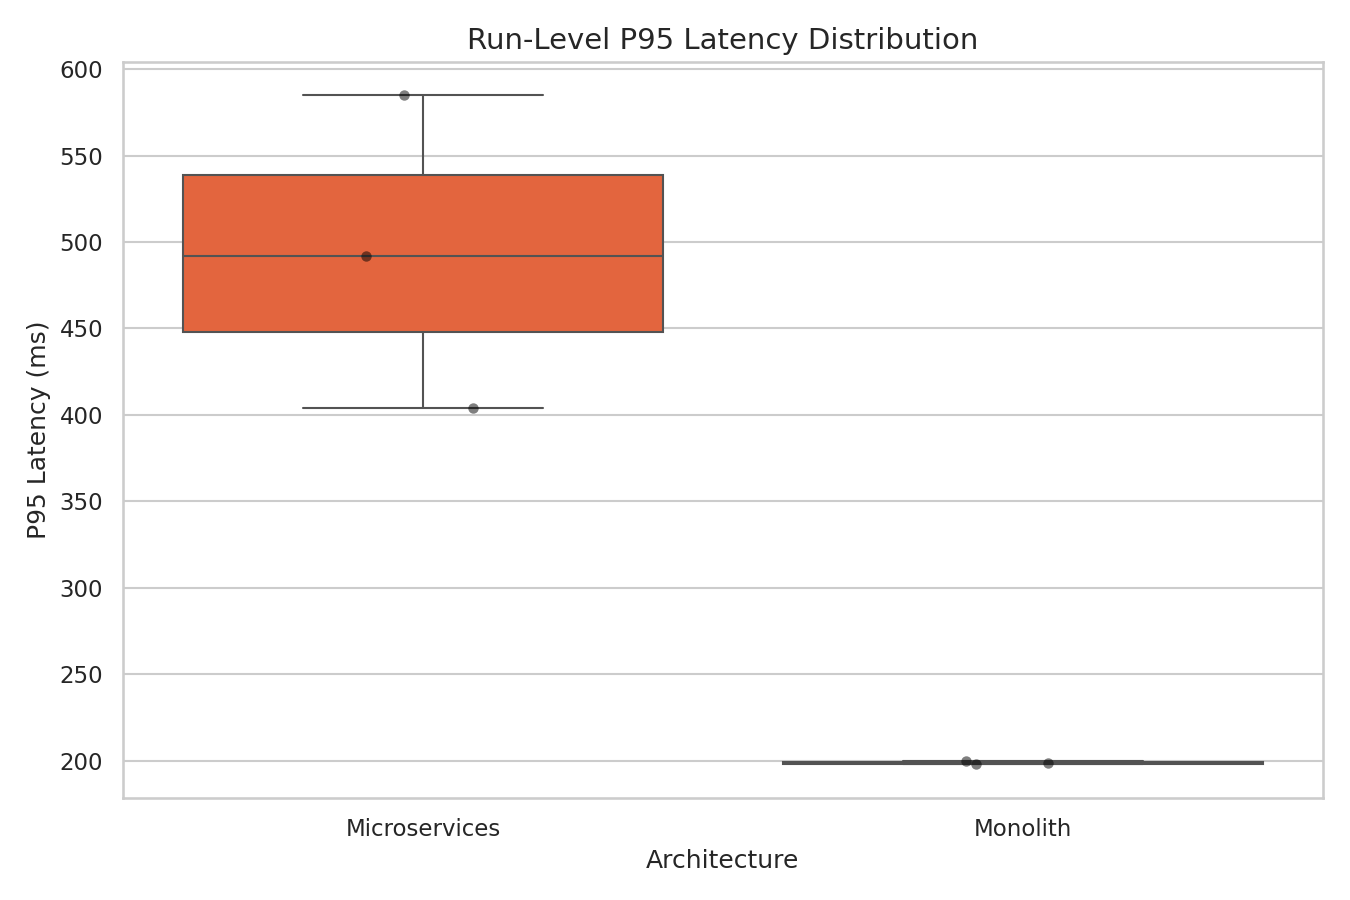
\includegraphics[width=\textwidth]{p95_latency_across_runs_boxplot.png}
	\caption{Baseline run-level P95 latency variability across repeated runs, the wider box confirms that microservices tail latency is not just higher on average but also less predictable run to run.}
	\label{fig-appendix-p95-boxplot}
\end{figure}

\FloatBarrier

\section*{Declarations}

\subsection*{Funding}

This research received no external funding.

\subsection*{Ethical approval}

Not applicable.

\subsection*{Informed consent}

Not applicable.

\subsection*{Author Contributions}

Bahaa El Deen Mohamed, Ahmad Louay, and Youssef Khaled, all contributed equally to study conception and design, implementation, experiment execution, data analysis, and manuscript preparation.
All authors read and approved the final manuscript.

\subsection*{Data Availability Statement}

Source code is available at \cite{repo_artifact}. Raw experiment artifacts (approximately 5.8 GB) are available from the corresponding author upon reasonable request due to size.

\subsection*{Conflict of Interest}

The authors declare that they have no conflict of interest.

\bibliographystyle{spbasic}
\bibliography{sn-bibliography}% common bib file

\end{document}
